\graphicspath{{sec/images/}{sec/code/s2/}}
\lstset{inputpath=sec/code/s2/}



\begin{frame}\relax \tW
    \centering\Huge \TeX\ boxes
\end{frame}


\begin{frame}[t, fragile]{``Horizontal'' boxes\tW}\relax

    \posesPicturesOverlayI{sec/code/s2}{hboxmy}{
            {38-38}{\ccol{\hbox} create box around the text. The box will never split in linebreak.}, 
            {38-40}{You can specify the length of the box with keyword \ccol{to}},
            {38-41}{You even can set the box to negative size},
            {38-41,44-45}{Another keyword, \ccol{spread} is the addition width},
            {38-41,44-47}{also both positive and negative}
            }

\skfootnote{\tugC{https://www.tug.org/utilities/plain/cseq.html\#hbox-rp}}

\end{frame}

\begin{frame}[fragile]{``Horizontal'' boxes\tW}{Usage}\relax
    \begin{columns}
    \begin{column}{0.4\textwidth}
     \verb|\hbox to -1pt{/}=|    
    \end{column}
    \begin{column}{0.4\textwidth}
         \hbox{\hbox to -1pt{/}=}
    \end{column}
    \end{columns}
    
    \begin{columns}
    \begin{column}{0.4\textwidth}
    \small
    \begin{minted}{latex}
\begin{tabbing}
\hbox to 4em{}\=\hbox to 4em{}\kill
a \> b\\
hello\> world!
\end{tabbing}
    \end{minted}     
    \end{column}
    \begin{column}{0.4\textwidth}
     \begin{tabbing}
          \hbox to 4em{}\=\hbox to 4em{}\kill
          a \> b\\
          hello\> world!
     \end{tabbing}
         
    \end{column}
    \end{columns}
     
\end{frame}

\begin{frame}[t]{``Vertical'' boxes\tW}{\TeX-way}\relax
    \posesPicturesOverlayI{sec/code/s2}{vboxmy}{
            {46-47}{\ccol{\vbox} create box around the text}, 
            {46-49}{You can specify the height of the box with keyword \ccol{to}},
            {46-49,52-55}{You even can set the box to negative size, use \ccol{spread}. But depth will remain the same},
            {46-49,52-55,58-59}{There is another box, \ccol\vtop},
            {46-49,52-55,58-61}{it will change the depth for you}
            }

    \skfootnote{\tugC{https://www.tug.org/utilities/plain/cseq.html\#vbox-rp}, \tugC{https://www.tug.org/utilities/plain/cseq.html\#vtop-rp}}
\end{frame}

\begin{frame}[t]{Move boxes\magicPage\tW}\relax
\posesPicturesOverlayI{sec/code/s2}{moveboxmy}{
    {39-39}{\ccol\raise\ and \ccol\lower\ for horizontal boxes}, 
    {39-39,41-46}{\ccol\moveleft\ and \ccol\moveright\ for vertical boxes}
}
     \skfootnote{\tugC{https://www.tug.org/utilities/plain/cseq.html\#raise-rp} \tugC{https://www.tug.org/utilities/plain/cseq.html\#lower-rp} \tugC{https://www.tug.org/utilities/plain/cseq.html\#moveleft-rp} \tugC{https://www.tug.org/utilities/plain/cseq.html\#moveright-rp}}
\end{frame}

\begin{frame}\relax \lW
\centering\Huge \LaTeX\ boxes
\end{frame}

\begin{frame}[t]{Horizontal boxes\lW}\relax
\posesPicturesOverlayI{sec/code/s2}{mboxmy}{
    {39-40}{\ccol\mbox\ and \ccol\makebox\ are like \ccol\hbox}, 
    {39-41}{\ccol\makebox\ has a width as an optional param},
    {39-41,43-46}{... and \ccol\makebox\ has text location as second optional param}
}
     \skfootnote{\lmanc{20.1}[179] \wikiC{https://en.wikibooks.org/wiki/LaTeX/Boxes\#makebox_and_mbox}}
\end{frame}

\inclassframe{
\begin{frame}[t]{Paragraph boxes\lW}\relax
\twocolImg{
% \lstinputlisting[linerange={1-10}]{parboxmyInc.tex}
\inputminted[firstline=1, lastline=10]{latex}{sec/code/s2/parboxmyInc.tex}
}{parboxmyInc}

% \ccol\parbox\ give you a box of text with some width and center vertical position.

% \inclassFrag{Add a \texttt{boxplay.sty} and wrap the \ccol\parbox\ with \ccol\boxingDim\string\parbox\{\...\}\{...\} or \ccol\boxingDimHug\string\parbox\{\...\}\{...\}}[-1]
\end{frame}}

\begin{frame}[t]{Paragraph boxes\lW\preMagicPage}\relax
\vspace*{-2ex}
\posesPicturesOverlayI{sec/code/s2}{parboxmy}{
    {44-44}{\ccol\parbox\ give you a box of text with some width. Also there are \ccol\pbox\ and \ccol{minipage} envirument}, 
    {44-44, 48-48}{It is just a box with  a big depth},
    {44-44, 48-50}{You can specify the position.\\ \ccol\parbox\ is useful when you want to put two lines to some command, that accepts only one line. Footnotes in the lectures use it.}
}
     \skfootnote{\lmanc{20.3}[181] \lmanc{8.18}{73} \wikiC{https://en.wikibooks.org/wiki/LaTeX/Boxes\#parbox,_minipage,_and_pbox}}
\end{frame}

\begin{frame}[fragile]{Boxes-modifiers\lW\magicPage}\relax
\twocolImg{
% \lstinputlisting[linerange={13-21, 25-25, 28-28}]{raiseboxmy.tex}
\inputminted[firstline=13, lastline=21]{latex}{sec/code/s2/raiseboxmy.tex}
\inputminted[firstline= 25, lastline=25]{latex}{sec/code/s2/raiseboxmy.tex}
\inputminted[firstline= 28, lastline=28]{latex}{sec/code/s2/raiseboxmy.tex}
}{raiseboxmy}
 
 \ccol\raisebox\verb|{lift}[height][depth]{text}| change the text position. \ccol{\rotatebox} rotates the text, \ccol\scalebox\ scales it
\skfootnote{\lmanc{20.4}[182] \lmanc{22.3.2}[198] \lmanc{22.3.3}[199] \wikiC{https://en.wikibooks.org/wiki/LaTeX/Boxes\#box_modifiers}}
\end{frame}

%%%%%%%%%%%%% manipulations %%%%%%%%%%%%%
\begin{frame}[fragile]{Box manipulation\lW}\relax
    
    \textbf{Define box} \ccol{\newsavebox\{\string\<boxname>\}}
    
    \textbf{Set box} \ccol{\savebox}
    
    \textbf{Provide the content without deleting it:} \ccol{\usebox}
    
    \textbf{Dimentions}: 
    \begin{enumerate}
        \item Create a length variable: \ccol\newlength
        \item Set the variable to dimention of the box CONTENT:
        \begin{itemize}
            \item width: \verb|\settowidth{\<len-var>}{\usebox{\<box>}}|
            \item height: \verb|\settoheight{\<len-var>}{\usebox{\<box>}}|
            \item depth: \verb|\settodepth{\<len-var>}{\usebox{\<box>}}|
        \end{itemize}
         
    \end{enumerate}
    
    \skfootnote{\lmanc{14.4-6}[133] \lmanc{20.5, 20.7}[183]}
\end{frame}

\begin{frame}{Box manipulation\lW}{Example}\relax

    \twocolImg{
    % \lstinputlisting[linerange={12-26}]{boxLaTeX.tex}
    \inputminted[firstline=12, lastline=26]{latex}{sec/code/s2/boxLaTeX.tex}
    }{boxLaTeX}
     
    \skfootnote{\ccol\the\ here is just to PRINT the length. Not the part of the command.}
\end{frame}




\begin{frame}{Box manipulation\tW}\relax

    \textbf{Define box} \ccol{\newbox\string\<boxname>}
    
    \textbf{Set box} \ccol{\setbox\string\<boxname>=<box>}
    
    \textbf{Provide the content without deleting it:} \ccol{\copy\string\<boxname>}
    
    \textbf{Provide the content with delete from memory:} \ccol{\box\string\<boxname>}
    
    \textbf{Dimentions}: width: \ccol\wd, height: \ccol\ht, depth: \ccol\dp
    
    \skfootnote{\knuthc{15}[131] }
\end{frame}

\begin{frame}{Box manipulation\tW}{Example}\relax

    \twocolImg{
    % \lstinputlisting[linerange={12-20}]{boxTeX.tex}
    \inputminted[firstline=12, lastline=20]{latex}{sec/code/s2/boxTeX.tex}
    }{boxTeX}
    
    \skfootnote{\ccol\the\ here is just to PRINT the length. Not the part of the command.}
\end{frame}


\inclassframe{

\begin{frame}{\exFrame{Implement footnotes}}{lvl 1}\relax
    Implement a footnote with the following behaviour (see illustration and a code to start with at the next slides):
    \begin{itemize}
        \item the footnote has ($2/3\cdot$ total width of the text) width 
        \item\relax <current frame number>/<total frame number> is located to the left (google how to add this in beamer!)
        \item\relax <the year after current year> is located to the right (you must use counters and increase the current year!)
    \end{itemize}
\end{frame}

\begin{frame}[t]{\exFrame{Implement footnotes}}{lvl 1}\relax
    \centering
    \vspace*{-1cm}
    \fbox{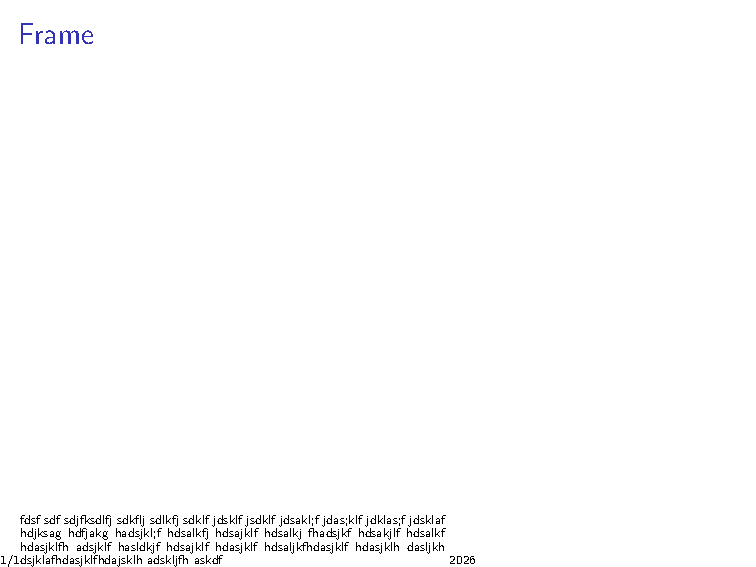
\includegraphics[scale=0.8]{exLvl1.pdf}}
\end{frame}

\begin{frame}{\exFrame{Implement footnotes}}{lvl 1}\relax
\vspace*{-1em} 
Use the following code as a base: 
     \inputminted{latex}{sec/code/s2/ex_prepere.tex}
\end{frame}

\begin{frame}{\exFrame{Implement footnotes}}{lvl 2}\relax
     Update the previous template. Make the following: if the text in footnote is higher than \textbf{30pt}, the footnote must becomes 1.5 times wider (google, how to compare two lengths!)
\end{frame}

}